\section{Definizione del prodotto}

% Nell'indice proposto da Tullio c'è:
% a. Metodo e formalismo di specifica
% b. Presentazione dell'architettura generale del sistema e identificazione dei componenti architetturali di alto livello

\subsection{Formalismo di specifica}

\subsection{Architettura di sistema}

\begin{figure}[H]
\centering
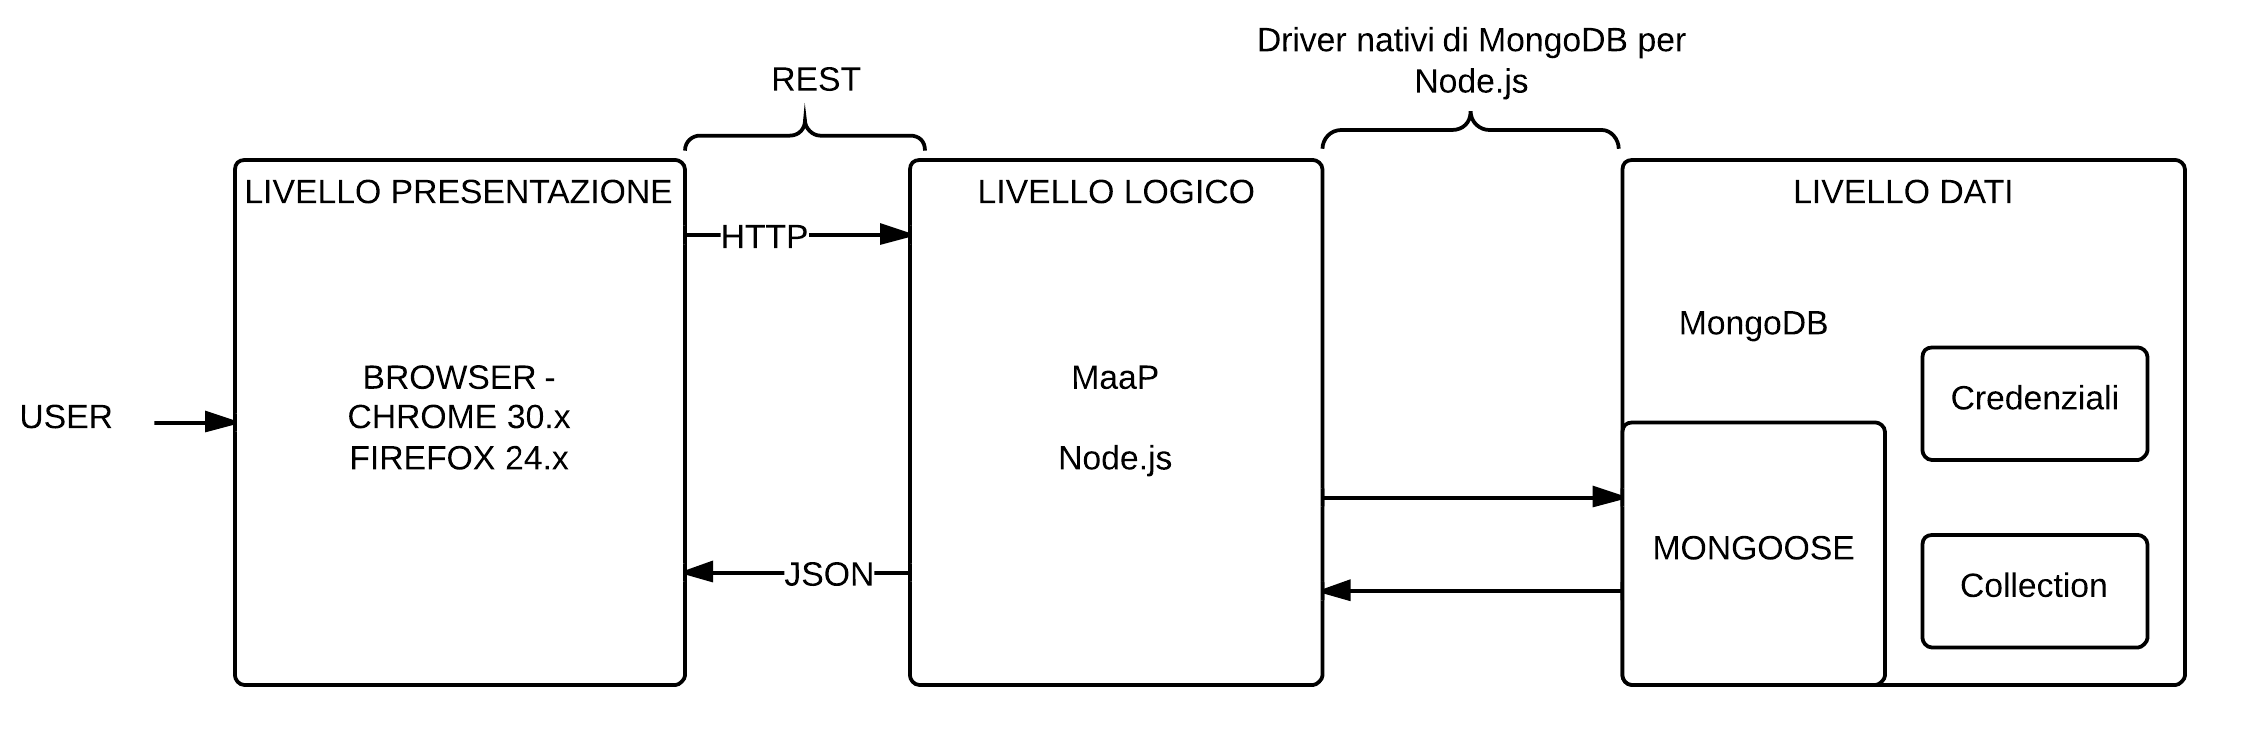
\includegraphics[scale=0.2]{3-TIER.png}
\caption{Schema del modello utilizzato \label{fig:architetturadisistema}}
\end{figure}

\subsection{Three-Tier Architecture}

\emph{Nota: Di seguito i termini modulo, strato e livello sono utilizzati come traduzione del termine inglese tier.}
 
Si tratta di un'architettura di tipo \glossario{client-server}, in cui i processi logici, la persistenza dei dati e l'interfaccia utente sono sviluppati e mantenuti in moduli tra loro indipendenti e distribuiti. Il vantaggio che ne consegue è che un modulo può essere aggiornato o sostituito senza dover alterare gli altri.

Come da figura \ref{fig:architetturadisistema} i tre livelli sono:
\begin{itemize}
\item \textbf{Livello presentazione} Si tratta dello strato che comunica con l'utente, il quale è estraneo all'esistenza degli altri moduli. Il compito di questo strato è fornire un'interfaccia utente, la quale comunicherà con il modulo logico per aggiornarsi e trasmettere le scelte dell'utente. Solitamente questo livello si trova sul \glossario{client};
\item \textbf{Livello logico} Questo livello racchiude le funzionalità, i processi e gli algoritmi dell'applicazione. Solitamente questo livello si trova su un \glossario{server} e si rapporta con il livello interfaccia e il livello dati; 
\item \textbf{Livello dati} In questo livello solitamente si trovano le \glossario{basi di dati}, che garantiscono la persistenza dei dati. È accessibile solo attraverso il livello logico, che ne garantisce la consistenza. In questo livello si trovano anche i componenti utili all'accesso della \glossario{base di dati}, nel nostro caso \glossario{Mongoose}.
E' importante far notare che uno strato dati può comunicare con più strati logici, che potranno utilizzare i dati in maniera diversa.
\end{itemize}

\glossario{Three-Tier} è l'architettura software scelta per \ProjectName.

\subsubsection{\glossario{REST}}

REST, ovvero Representational State Transfer è un tipo di \glossario{RPC}. Si basa su un protocollo di comunicazione \glossario{stateless} di tipo client-server, e solitamente tale protocollo è \glossario{HTTP}, che è stato scelto anche per \ProjectName.

I motivi che hanno spinto alla scelta di REST sono:
\begin{itemize}
\item Semplicità di utilizzo;
\item Indipendenza dal sistema operativo utilizzato dal \glossario{client};
\item Indipendenza dai linguaggi di programmazione utilizzati;
%\item In coppia con HTTPS permette una certa sicurezza delle comunicazioni.
\end{itemize}

\glossario{REST} utilizza il concetto di risorsa, ovvero un aggregato di dati con un nome (\glossario{URI}) e una rappresentazione, su cui è possibile invocare le operazioni \glossario{CRUD} tramite il protocollo sopracitato.

Nell'\glossario{URI} inviato sono presenti il nome della risorsa e la sua rappresentazione, identificata dall'estensione del file scelto, e per \ProjectName è stato scelto il formato \glossario{JSON}, in quanto il suo \glossario{parsing} in \glossario{JavaScript} è più semplice rispetto, ad esempio, quello di \glossario{XML} o \glossario{CSV}.

Un'altra caratteristica di \glossario{REST} è che essendo \glossario{stateless} ogni richiesta dovrà contenere tutte le informazioni necessarie e non dipende dallo stato del sistema.

\subsection{Tecnologie utilizzate}
L'architettura è stata progettata cercando di tenere in considerazione diverse tecnologie, alcune delle quali espressamente richieste nel capitolato d'appalto. Vengono di seguito elencate e descritte le principali tecnologie impiegate e le motivazioni del loro utilizzo.

\begin{itemize}
	\item \textbf{Node.js} per la realizzazione della componente server;
	\item \textbf{Express.js} per la realizzazione dell’infrastruttura della web application generata;
	\item \textbf{MongoDB}: database di tipo NoSQL per la parte di recupero e salvataggio dei dati;
	\item \textbf{Mongoose} per l’interfacciamento con il database;
	\item \textbf{AngularJS} per gestire il rendering dell'interfaccia grafica lato client.
\end{itemize}


\subsubsection{Node.js}
\textbf{Node.js} è un \glossario{framework} per realizzare applicazioni Web veloci e scalabili in JavaScript, permettendo di utilizzare questo linguaggio, tipicamente utilizzato nel lato client, anche per la scrittura di applicazioni lato server.
La piattaforma è basata sul runtime di Google \glossario{V8 JavaScript Engine} utilizzato anche da \glossario{Chrome} e disponibile sulle principali piattaforme.

I principali vantaggi derivati dall'utilizzo di Node.js sono:
\begin{itemize}
	\item \textbf{Approccio asincrono}: Node.js permette di accedere alle risorse del sistema operativo in modalità event-driven e non sfruttando il classico modello basato su processi o thread concorrenti, utilizzato dai classici web server. Ciò garantisce una maggiore efficienza in termini di prestazioni poiché durante le attese, il runtime può gestire qualcos’altro in maniera asincrona.
	\item \textbf{Architettura modulare}: Lavorando con Node.js è molto facile organizzare il lavoro in librerie, importare i moduli e combinarli fra loro. Questo è reso molto comodo attraverso il node package manager (npm) attraverso il quale lo sviluppatore può contribuire e accedere ai package messi a disposizione dalla community.
\end{itemize}

\subsubsection{Express.js}
\textbf{Express.js} è un \glossario{framework} minimale per creare applicazioni Web con Node.js. Richiede moduli Node di terze parti per applicazioni che prevedono l’interazione con la basi di dati; \newline
\`E stato utilizzato il \glossario{framework} Express.js per supportare lo sviluppo dell'application server grazie alle utili e robuste features da esso offerte, le quali sono pensate per non oscurare le funzionalità fornite da Node.js aprendo così le porte all'utilizzo di moduli per Node.js atti a supportare specifiche funzionalità.

\subsubsection{MongoDB}
\textbf{MongoDB} è un database NoSQL open-source scalabile e altamente performante di tipo document-oriented, ovvero in cui i dati sono archiviati sotto forma di documenti in stile \glossario{JSON} con schemi dinamici, secondo una struttura molto semplice e potente.

I principali vantaggi derivati dal suo utilizzo sono:
\begin{itemize}
	\item \textbf{Alte performance}: non ci sono join che possono rallentare le operazioni di lettura o scrittura. L’indicizzazione include gli indici di chiave anche sui documenti innestati e sugli array permettendo una rapida interrogazione al database;
	\item \textbf{Affidabilità}: alto meccanismo di replicazione su server;
	\item \textbf{Schemaless}: non esiste nessuno schema, è più flessibile e può essere facilmente trasformato in oggetti;	
	\item Permette di definire query complesse utilizzando un linguaggio che non è \glossario{SQL};
	\item Permette di processare parallelamente i dati (\glossario{Map-Reduce});
	\item Tipi di dato più flessibili.
\end{itemize}

\subsubsection{Mongoose}
\textbf{Mongoose} è una libreria per MongoDB che permette di definire degli schemi per modellare i dati del database, facendo rispettare una certa struttura ai dati per la creazione di nuovi Document. Inoltre, fornisce molti strumenti utili per la validazione dei dati, per la definizione di query e per il cast dei tipi predefiniti.

Per interfacciare l'application server con MongoDB, sono disponibili diversi progetti open-source. Per questo progetto è stato scelto di utilizzare Mongoose, attualmente il più diffuso.	
